\documentclass{acm_proc_article-sp}
%\documentclass{sig-alternate}

% Set letter paper size:
%\setlength{\paperheight}{11in}
%\setlength{\paperwidth}{8.5in}

\usepackage{authblk}
%\renewcommand\Authfont{\small}
%\renewcommand\Affilfont{\itshape\footnotesize}

\usepackage{times,amsmath,epsfig}
\usepackage[hyphens]{url}
\usepackage[pagebackref=true]{hyperref}
%\usepackage[hang,raggedright]{subfig}
%\usepackage[font=footnotesize]{subfig}
\usepackage{subfig}
\usepackage{amsmath, graphicx}
%\usepackage{multiFloats}
\usepackage{url}
\usepackage{verbatim}
\usepackage{amssymb,amsmath}
\usepackage{alltt}
%\usepackage{pslatex}
%\usepackage[all]{xy}
\usepackage{color}
\usepackage{listings}

\newcommand\F[1]{\textcolor{red}{F: #1}}
\newcommand\K[1]{\textcolor{red}{K: #1}}
\newcommand\R[1]{\textcolor{red}{R: #1}}

\begin{document}
%\sloppy
%\thispagestyle{empty}
\title{\textbf{Information Loss During Size Reduction Depending On Structure Scale}}

\author[1]{Laurens Bogaardt}
\author[1]{Romulo Goncalves}
\author[2]{Raul Zurita-Milla}
\author[2,3]{Emma Izquierdo-Verdiguier}

\affil[1]{NLeSC Amsterdam, The Netherlands \vspace{1pt} \{\emph{\{l.bogaardt, r.goncalves\}@esciencecenter.nl}\}}%, o.rubi\}@esciencecenter.nl}\}}
\affil[2]{Faculty of Geo-Information Science and Earth Observation (ITC), University of Twente, the Netherlands \vspace{10pt} \{\{\emph{\{r.zurita-milla,e.izquierdoverdiguier\}@utwente.nl}\}\}}
\affil[3]{Image Processing Laboratory (IPL), Universitat de Valencia, Spain}

\date{} % <--- leave date empty
\maketitle\thispagestyle{empty} %% <-- you need this for the first page

\begin{abstract}
Lorem Ipsum is simply dummy text of the printing and typesetting industry. Lorem Ipsum has been the industry's standard dummy text ever since the 1500s, when an unknown printer took a galley of type and scrambled it to make a type specimen book. It has survived not only five centuries, but also the leap into electronic typesetting, remaining essentially unchanged. It was popularised in the 1960s with the release of Letraset sheets containing Lorem Ipsum passages, and more recently with desktop publishing software like Aldus PageMaker including versions of Lorem Ipsum.
\end{abstract}

\section{Introduction}
\label{sec:Introduction}

In this article, we will reduce the size of datasets representing Gaussian Random Fields using various techniques and investigate how much information is lost. These techniques can be useful when the original dataset is very large and performing analyses on it is costly.

\subsection{CCA and Related Analyses}
\label{sec:Introduction CCA and Related Analyses}

In an MCA, modes are found where the left- and the right-field covary maximally (1992 - Bretherton, Smith, Wallace). One technique to find these modes is to perform an SVD on the product of the datasets. That is why the term SVD is often used synonymously with MCA.
In an CCA, modes are found where the left- and the right-field correlate maximally. In practice, the datasets are first standardized before multiplied and decomposed. MCA and CCA are very much related, but the resulting modes and vectors need not be the same (1992 - Bretherton, Smith, Wallace).
In a PCA, the first and the second dataset are identical. Whether to maximize the covariance or the correlation depends on whether the units of each vector is the same.

\subsection{Pre-processing}
\label{sec:Introductio Pre-processingn}

It has been suggested that filtering data for noise is important before the statistical analysis (1987 - Barnett, Preisendorfer). This is because any statistical analysis will choose its regression-coefficients so as to optimize the fit. It may occur that two noise-vectors in the two fields coincidentally covary. In a CCA, where the fields are standardized, this resulting mode may appear important even though it stems from noise. In an MCA, the variance of the noise will be low, so the chance that it will appear as an important mode is less (1992 - Bretherton, Smith, Wallace). One method of finding the right level of filtering is by bootstrapping/cross-validating the results (1999 - Livezey, Smith).
A second type of pre-processing relates to weighting the input data (1999 - Livezey, Smith). One reason to weight spatial data is to undo the effect of the curvature of the Earth. When comparing two datasets with different number of spatial points can it also be important to weight data.

\subsection{QR-Decomposition and Projections}
\label{sec:Introduction QR-Decomposition and Projections}

By rotating (projecting) rectangular matrices, the action can be captured by a square matrix with dimensions equal to that of the smallest dimension of the original, rectangular matrix. This can be done with a QR-decomposition, where R is a square matrix and Q a projection matrix. It can also be done via an SVD, where the original matrix is decomposed into U, S and V. The product of S and V gives a square matrix, with S the projection matrix.

\subsection{Post-processing and Model Assessment}
\label{sec:Introduction Post-processing and Model Assessment}

Any rotation or projection applied in the pre-processing step to the datasets must be undone. Furthermore, the resulting model must be assessed. This can be done using bootstrapping/cross-validation (1999 - Livezey, Smith).

\subsection{Gaussian Random Spatial Field}
\label{sec:Introduction Gaussian Random Spatial Field}

The singular values of a matrix represent the amount of variance in the original dataset explained by the associated singular vector. The explainedVariance function takes the list of singular values and returns a list of explained variance. This can e.g. be used in a plot.

The $\alpha$ is a measure of the spatial autocorrelation of the field. In particular, fields with large scale structure have a more negative $\alpha$. Additionally, the size of the singular values can be plotted. This is related to the power spectrum and will also provide information about the scale of the structure in the field. Fianlly, there are other measures of spatial autocorrelation. These include the Gamma Index and Moran's I. The Python module pysal contains functions to calculate these values. We will include them for each plot.

\begin{figure}[h]
\begin{center}
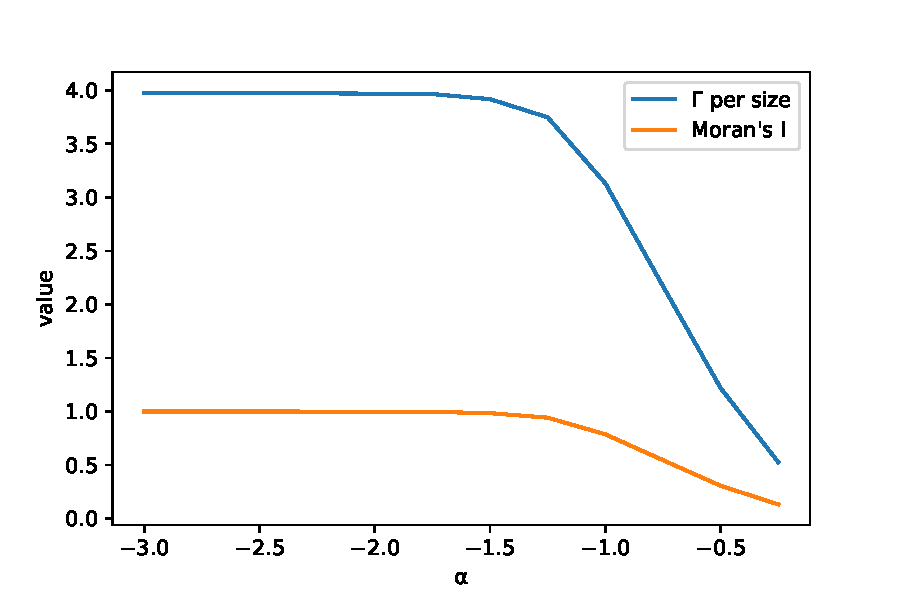
\includegraphics[scale=0.5]{Results/plotGammaAndMoransI.pdf}
\caption[Small caption]{Caption}
\label{fig:plotGammaAndMoransI}
\end{center}
\end{figure}

When $\alpha$ is less negative, the Gaussian Random Field has smaller scale structure. It is closer to randomness and has less autocorrelation. As expected, this can be seen in the two measures of autocorrelation, which are now smaller.

\subsection{Gaussian Random Spatial-Temporal Field}
\label{sec:Introduction Gaussian Random Spatial-Temporal Field}

In many real-world applications, the analysis of a field does not only involve a single time snapshot. In fact, it often includes data over multiple weeks, months or years, where the field over the entire time period does not change drastically. Just as there is spatial autocorrelation, there is temporal autocorrelation. In principle, there can be a different level of correlation over time than over space. However, for simplicity, we are using the same $\alpha$ determine the level of autocorrelation in all dimensions.

\section{Techniques}
\label{Techniques}

This section will discuss four techniques to analyse large datasets efficiently using SVD.

\subsection{Exact Norm Difference via SVD}
\label{sec:Techniques Exact Norm Difference via SVD}

In real-world application, one often wants to find the norm of the difference between two fields. This can be done by subtracting one matrix from the other and calculating the norm. However, for large matrices, this can be inefficient. Performing an SVD of both matrices can reduce the internal calculations. The normDifferenceFromUSVs function can take such input SVDs and determine the norm of their difference in an efficient manner, provided the number of singular values is small. The result is mathematically identical to the full calculation, which means that any error will be of the order of machine-precision.

\begin{figure}[h]
\begin{center}
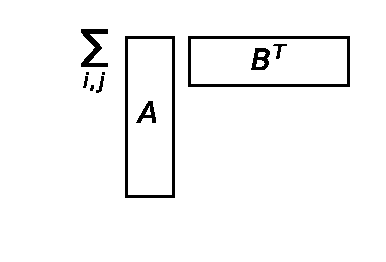
\includegraphics[scale=0.25]{Results/normDifferenceFromUSVs.pdf}
\caption[Small caption]{Caption}
\label{fig:normDifferenceFromUSVs}
\end{center}
\end{figure}

Lorem Ipsum is simply dummy text of the printing and typesetting industry. Lorem Ipsum has been the industry's standard dummy text ever since the 1500s, when an unknown printer took a galley of type and scrambled it to make a type specimen book. It has survived not only five centuries, but also the leap into electronic typesetting, remaining essentially unchanged. It was popularised in the 1960s with the release of Letraset sheets containing Lorem Ipsum passages, and more recently with desktop publishing software like Aldus PageMaker including versions of Lorem Ipsum.

\subsection{Exact SVD via QR Decomposition}
\label{sec:Techniques Exact SVD via QR Decomposition}

In real-world application, one often wants to find the relation between two fields. This can be done by performing an SVD of the cross-correlation matrix of these two fields. In particular, the two input datasets often have the various gridpoint as rows and will have the sample of recorded values over time as columns. Multiplying these gives the cross-correlation matrix. However, for highly rectangular matrices, when there are many spatial gridpoint but few temporal samples, the resulting cross-correlation matrix is inefficiently large. The qrProductSVD function can take such input data and perform an SVD in an efficient manner. The result is mathematically identical to the full SVD, which means that the difference will be at machine-precision.

\begin{figure}[h]
\begin{center}
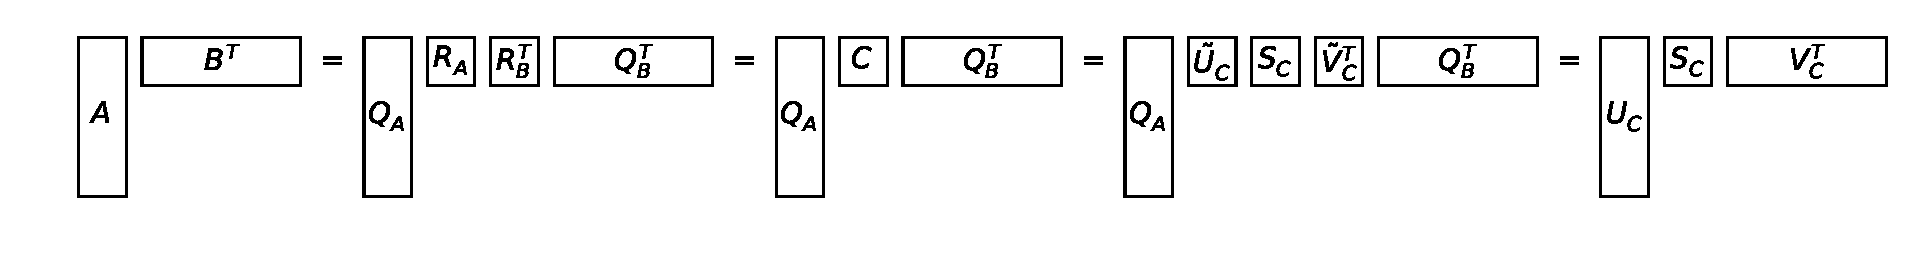
\includegraphics[scale=0.25]{Results/qrProductSVD.pdf}
\caption[Small caption]{Caption}
\label{fig:qrProductSVD}
\end{center}
\end{figure}

Lorem Ipsum is simply dummy text of the printing and typesetting industry. Lorem Ipsum has been the industry's standard dummy text ever since the 1500s, when an unknown printer took a galley of type and scrambled it to make a type specimen book. It has survived not only five centuries, but also the leap into electronic typesetting, remaining essentially unchanged. It was popularised in the 1960s with the release of Letraset sheets containing Lorem Ipsum passages, and more recently with desktop publishing software like Aldus PageMaker including versions of Lorem Ipsum.

\subsection{Approximate SVD via Spatial Coarsening}
\label{sec:Techniques Approximate SVD via Spatial Coarsening}

Although the qrProductSVD function works well for two rectangular matrices, sometimes the input data is large and square. Performing an SVD on such a large dataset will be time consuming and, perhaps, inefficient given the desired level of precision. When a field have large scale structure, the values of neighbouring cells do not change drastically. This is what autocorrelation means. As such, perhaps neighbouring cells can be averaged together to produce a smaller dataset which still faithfully describes the original field. The matrixToGrid function can cut a matrix into multiple smaller sections.


\begin{figure}[h]
\begin{center}
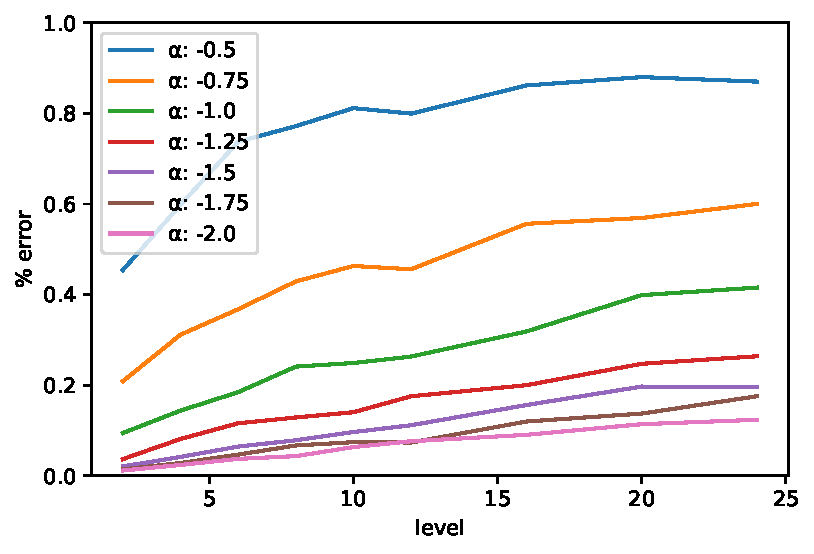
\includegraphics[scale=0.5]{Results/plotSingleSpatialFieldViaCoarsening.pdf}
\caption[Small caption]{Caption}
\label{fig:plotSingleSpatialFieldViaCoarsening}
\end{center}
\end{figure}

The testProductSpatialTemporalFieldsViaCoarsening function determines the percentage of the information lost in a coarsening process for matrices of various sizes and $\alpha$'s, and at various levels of coarsening. The two input matrices used here are similar, as they are generated by the same Gaussian Random Process. Therefore, they will correlate highly and the bases in which they are best described will be similar. In principle, any two datasets can be analysed and the amount of information lost during the coarsening process will likely depend on the similarity between the two datasets. This is one aspect which we do not cover here and leave for further research.

Due to the multiplication step in this analysis, the typical error due to coarsening is larger than before. As before, $\alpha$ plays an important part, with more negative $\alpha$'s leading to a less dramatic loss in information due to coarsening.

\begin{figure}[h]
\begin{center}
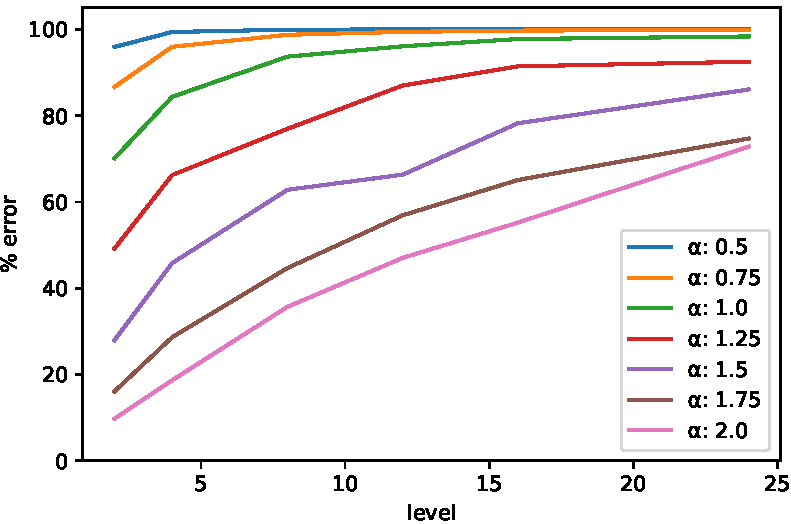
\includegraphics[scale=0.5]{Results/plotProductSpatialTemporalFieldsViaCoarsening.pdf}
\caption[Small caption]{Caption}
\label{fig:plotProductSpatialTemporalFieldsViaCoarsening}
\end{center}
\end{figure}

The additional benefit of coarsening is that data collection can be optimised.

\subsection{Approximate SVD via Dimensionality Reduction}
\label{sec:Techniques Approximate SVD via Dimensionality Reduction}

The spatial coarsening process is intuitive and easy to implement. It is not, however, the most efficient way to reduce the size of a dataset. Dimensionality reduction refers to discarding modes which contribute little to the variance in a dataset. An SVD is precisely the procedure used to find modes which explain as much variance as possible. Discarding the smallest singular values/vectors is, therefore, the most efficient form of dimensionality reduction. Performing an SVD on a large dataset, however, is computationally costly. The Randomised Dimensionality Reduction process is far more efficient.

The reduceSizeRandomisedSquare function reduces the input matrix to a smaller square matrix of l by l. It also gives two projection matrices which can bring the rows and columns of this smaller matrix back to the bases of the original input. To make the result more precise, the procedure can be repeated multiple times. The parameter i indicates how many loops are performed.

\begin{figure}[h]
\begin{center}
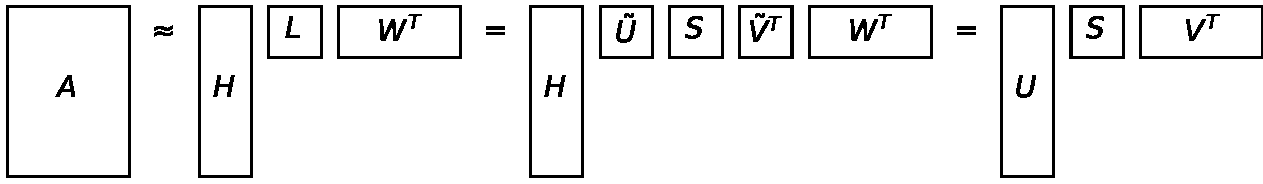
\includegraphics[scale=0.25]{Results/reduceSizeRandomisedSquare.pdf}
\caption[Small caption]{Caption}
\label{fig:reduceSizeRandomisedSquare}
\end{center}
\end{figure}

As seen, it is possible for some fields to be represented by matrices of much smaller sizes without losing any substantial amount of information. This is obvious when one realises the singular modes which are removed during the reduction are the smallest ones, described by the tail-end of the power law. In the review article by Halko, Martinsson and Tropp on randomised dimensionality reduction, it is suggested to oversample the reduction. This is because the error introduced in the process is of the same order as the size of the last sampled singular value. If one is interested in the k dominant modes, reducing to a k + l, for some small l, rank approximation will ensure the first k modes are approximated quite well. Indeed, as seen below, the more modes one is interested in, the larger the difference compared with the original matrix.

The Randomised Dimensionality Reduction process can also be applied to the CCA or MCA analysis of two spatial-temporal fields. Similar to the QR Product SVD, it has the advantage that the SVD is applied to a small l x l matrix. The result will be an approximation, but, as we will see, can be close to the real solution.

\begin{figure}[h]
\begin{center}
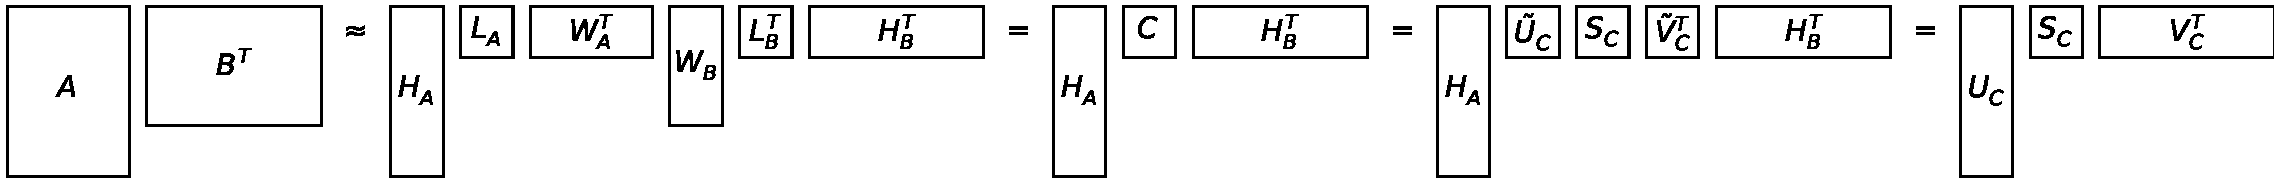
\includegraphics[scale=0.2]{Results/randomisedSquareProductSVD.pdf}
\caption[Small caption]{Caption}
\label{fig:randomisedSquareProductSVD}
\end{center}
\end{figure}

To see the effect of dimensionality reduction on such a matrix product, let's generate two Gaussian Random Fields and plot their corss-correlation matrix together with a reduced version. To determine precisely how much information is lost during the reduction, we should look at the variance of the datasets. The norm of the difference between the reduced matrix and the original is the amount of information lost in the reduction process.


\begin{figure}[h]
\begin{center}
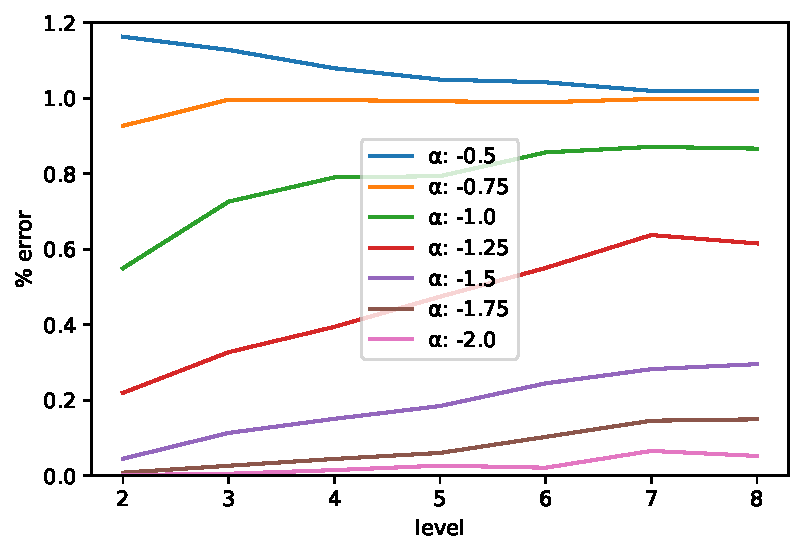
\includegraphics[scale=0.5]{Results/plotRandomisedSizeReducedMatrixProduct.pdf}
\caption[Small caption]{Caption}
\label{fig:plotRandomisedSizeReducedMatrixProduct}
\end{center}
\end{figure}

The testRandomisedSizeReducedMatrixProduct function determines the percentage of the information lost in a reduction process for matrices of various sizes and $\alpha$'s, and at various levels of reduction. The two input matrices used here are similar, as they are generated by the same Gaussian Random Process. Therefore, they will correlate highly and the bases in which they are best described will be similar. In principle, any two datasets can be analysed and the amount of information lost during the coarsening process will likely depend on the similarity between the two datasets. This is one aspect which we do not cover here and leave for further research.

Due to the multiplication step in this analysis, the typical error due to reduction is larger than before. There is an affect of temporal size on the information loss. The randomisedSquareProductSVD function is especially useful for square input matrices. To be able to do the comparisons with the full SVD quickly, we use rectangular matrices here. The larger the temporal size, the more square the input matrices. As before, the scale of the structure of the field influences the information loss. The effect in this case can be quite dramatic. Especially for more negative $\alpha$, this procedure performs much better than the coarsening procedure.

Note that, unlike the coarsening procedure, the reduction is not applied on each time-slice of the spatial field, but rather on the spatially-flattened time-series. Therefore, the level of spatial auto correlation may not be as important as the level of temporal auto correlation. The proper analysis of this is left for further research.

The reduction of the number of dimensions of each input dataset is actually advised by some researcher to combat noisy data.

\section{Applications}
\label{Applications}

Lorem Ipsum is simply dummy text of the printing and typesetting industry. Lorem Ipsum has been the industry's standard dummy text ever since the 1500s, when an unknown printer took a galley of type and scrambled it to make a type specimen book. It has survived not only five centuries, but also the leap into electronic typesetting, remaining essentially unchanged. It was popularised in the 1960s with the release of Letraset sheets containing Lorem Ipsum passages, and more recently with desktop publishing software like Aldus PageMaker including versions of Lorem Ipsum.

\subsection{Approximate SVD via Spatial Coarsening}
\label{sec:Applications Approximate SVD via Spatial Coarsening}

Lorem Ipsum is simply dummy text of the printing and typesetting industry. Lorem Ipsum has been the industry's standard dummy text ever since the 1500s, when an unknown printer took a galley of type and scrambled it to make a type specimen book. It has survived not only five centuries, but also the leap into electronic typesetting, remaining essentially unchanged. It was popularised in the 1960s with the release of Letraset sheets containing Lorem Ipsum passages, and more recently with desktop publishing software like Aldus PageMaker including versions of Lorem Ipsum.

\subsection{Approximate SVD via Dimensionality Reduction}
\label{sec:Applications Approximate SVD via Dimensionality Reduction}

Lorem Ipsum is simply dummy text of the printing and typesetting industry. Lorem Ipsum has been the industry's standard dummy text ever since the 1500s, when an unknown printer took a galley of type and scrambled it to make a type specimen book. It has survived not only five centuries, but also the leap into electronic typesetting, remaining essentially unchanged. It was popularised in the 1960s with the release of Letraset sheets containing Lorem Ipsum passages, and more recently with desktop publishing software like Aldus PageMaker including versions of Lorem Ipsum.

\section{Further Questions}
\label{Further Questions}

It may be interesting to extend this research to fields other than the Gaussian Random Field. This type was chosen because its structure scale can be captured in a single parameter $\alpha$. In many applications, however, the dataset does not resemble such a Gaussian Random Field.

Additionally, it would be an improvement to relax the assumption that the auto-correlation in the time direction is similar to that in the spatial directions. In fact, it may even be more realistic to have different levels of auto correlation in the $x$ and in the $y$ direction.

{
\footnotesize
\bibliographystyle{abbrv}
%\phantomsection
%\label{sec:Bibliography}
\bibliography{Bibliography}
}

\end{document}
